% ============================================================
%  SlangGPT — AIE241 NLP Course Paper
%  Compiler: XeLaTeX (required for Arabic script)
% ============================================================
\documentclass[11pt]{article}

\usepackage[margin=0.5in, columnsep=0.25in]{geometry}
\usepackage{fontspec}
\usepackage{polyglossia}
\usepackage{amsmath}
\usepackage{amssymb}
\usepackage{booktabs}
\usepackage{multirow}
\usepackage{array}
\usepackage{float}
\usepackage{graphicx}
\usepackage{caption}
\usepackage{subcaption}
\usepackage{hyperref}
\usepackage{xcolor}
\usepackage{enumitem}
% Fix paragraph formatting
\setlength{\parindent}{0pt}
\setlength{\parskip}{0.4\baselineskip}
\sloppy
% Arabic support - English as main language!
\setmainlanguage{english}
\setotherlanguage{arabic}
\newfontfamily\arabicfont[Script=Arabic]{Amiri}
\newcommand{\arb}[1]{{\arabicfont\beginR #1\endR}}

\hypersetup{
    colorlinks=true,
    linkcolor=blue,
    urlcolor=blue,
    citecolor=blue
}

\title{\textbf{SlangGPT: Fine-tuning AraGPT-2 for Egyptian Arabic\\
Dialect-to-Modern Standard Arabic Translation and Detection}}

\author{
  Abdelrahman Ahmed \\
  Department of Artificial Intelligence \\
  AIU University \\
  \texttt{abdelrahman.younes.2024@aiu.edu.eg}
  \and
  Adham Ashraf \\
  Department of Artificial Intelligence \\
  AIU University \\
  \texttt{adham.helmy.2024@aiu.edu.eg}
  \and
  Ahmed Fekry \\
  Department of Artificial Intelligence \\
  AIU University \\
  \texttt{ahmad.mansour.2024@aiu.edu.eg}
}

\date{}

\begin{document}
\maketitle

\begin{abstract}

\noindent Pretrained Arabic language models must be adapted to handle the significant linguistic gap between Egyptian Arabic dialect and Modern Standard Arabic (MSA). In this project, we investigate how a pretrained AraGPT-2 model can be fine-tuned to perform both generation and classification tasks on Egyptian Arabic. Inspired by the Stanford CS224N framework of Hernandez and Naik \cite{hernandez2025}, which extended GPT-2 for informal and slang-aware language understanding, we adapt their methodology to the Arabic dialect setting.

\noindent For dialect-to-MSA generation, we fine-tune AraGPT-2 as a conditional autoregressive language model to produce formal Arabic continuations given an Egyptian Arabic input. For dialect detection, we adapt a cloze-style prompting formulation using AraGPT-2's last-token hidden state to classify whether a candidate MSA sentence is a correct translation of a given Egyptian Arabic input.

\noindent Our results show that fine-tuning substantially improves performance on both tasks. The generation model achieves a chrF score of 29.08 and BLEU of 6.63, compared to zero-shot baselines of 10.62 and 0.02 respectively. The detection model achieves 0.956 accuracy on both development and test sets, compared to a 0.500 zero-shot baseline. These results demonstrate that transformer-based Arabic language models can be effectively adapted to informal dialect processing through targeted fine-tuning, even with a moderately sized dataset.
\end{abstract}

%───────────────────────────────────────────────────────────────────
\section{Key Information}
\begin{itemize}[noitemsep]
  \item \textbf{Course:} (AIE241) Natural Language Processing
  \item \textbf{Supervisor:} Ashraf Elsayed
  \item \textbf{Dataset:} AdhamAshraf/egyptian-2-arabic \cite{ashraf2026} —
        18,250 Egyptian Arabic / MSA parallel sentence pairs
  \item \textbf{Repository:} \url{https://github.com/adhamashraf7788/SlangGPT}
  \item \textbf{HuggingFace:} \url{https://huggingface.co/datasets/AdhamAshraf/egyptian-2-arabic}
  \item \textbf{Kaggle:} \url{https://www.kaggle.com/datasets/adhamashraf77/egyptian-2-arabic}
\end{itemize}

%───────────────────────────────────────────────────────────────────
\section{Introduction}

Arabic is not a monolithic language. The variety spoken daily by over 100 million Egyptians — Egyptian Arabic — differs substantially from Modern Standard Arabic (MSA), the formal written register used in media, literature, and official communication. This gap creates a persistent challenge for Arabic NLP systems: models trained on MSA corpora often fail to understand, normalize, or respond appropriately to dialectal input \cite{habash2010}.

Egyptian Arabic is characterized by distinct phonological reductions (e.g., \textit{مش} for \textit{ليس}), borrowed vocabulary (e.g., \textit{أوكيه}), shortened interrogatives (e.g., \textit{إيه} for \textit{ماذا}), and pragmatic particles that carry emotional tone without direct MSA equivalents. These features make Egyptian Arabic both challenging and important for dialect-aware NLP: any assistant, translation system, or text normalization tool that encounters Egyptian users must handle this register gracefully.

This project builds directly on the framework of Hernandez and Naik \cite{hernandez2025}, who investigated fine-tuning GPT-2 for informal slang understanding in English, including Gen-Z slang detection and generation. We extend their approach to the Arabic dialect setting by replacing the English GPT-2 backbone with AraGPT-2 \cite{antoun2021}, an Arabic-native transformer pretrained on large Arabic web corpora, and replacing the English slang dataset with a parallel Egyptian Arabic / MSA corpus.

We study two tasks: \textbf{dialect-to-MSA generation}, where the model produces a formal Arabic translation of an Egyptian input, and \textbf{dialect detection}, where the model classifies whether a candidate MSA sentence is a correct translation of a given Egyptian Arabic utterance. Together these tasks mirror the generation and detection framework of Hernandez and Naik, adapted for the Arabic dialect setting.

%───────────────────────────────────────────────────────────────────
\section{Related Work}

\paragraph{Arabic dialect NLP and pretrained models.}
Arabic dialect processing has received growing attention in NLP. Habash \cite{habash2010} provides foundations for computational dialect processing, while Darwish et al.\ \cite{darwish2021} and Zalmout and Habash \cite{zalmout2017} address dialect identification and morphological tagging for Egyptian Arabic. Antoun et al.\ \cite{antoun2021} introduced AraGPT-2, trained on 77GB of Arabic text, which is the backbone of our models. The same group introduced AraBERT \cite{antoun2020}, demonstrating that Arabic-specific pretraining substantially outperforms multilingual models.

\paragraph{Informal language and the Stanford framework.}
Sun et al.\ \cite{sun2024} show that informal linguistic variation poses significant challenges for pretrained models, motivating task-specific fine-tuning. Hernandez and Naik \cite{hernandez2025} demonstrated that GPT-2 can be fine-tuned for slang detection and generation through cloze-style prompting, achieving 0.965 accuracy on Gen-Z slang detection versus a 0.500 zero-shot baseline. Our work directly extends this methodology to Arabic dialect.
%───────────────────────────────────────────────────────────────────
\section{Approach}

Our project adapts the AraGPT-2 architecture to two downstream tasks: dialect-to-MSA generation and dialect-translation detection. In all experiments we fine-tune pretrained AraGPT-2 models using the AdamW optimizer with cosine or linear learning rate scheduling.

\subsection{Baselines}

As baselines, we evaluate zero-shot AraGPT-2 on both tasks without any task-specific fine-tuning. For generation, the zero-shot model is prompted with the template:

\begin{center}
\texttt{dialect: \{input\} $\hookleftarrow$ msa:}
\end{center}
and generates a continuation autoregressively. For detection, the zero-shot model encodes the full cloze prompt and the predicted label is determined by comparing the vocabulary logits for the tokens corresponding to \arb{نعم} (yes) and \arb{لا} (no).

The zero-shot generation baseline achieves a chrF score of 10.62 and BLEU of 0.02, with a perplexity of 11,851,030 on the test set — reflecting the severe domain mismatch between the base model's web training distribution and the parallel translation task. The zero-shot detection baseline achieves 0.500 accuracy, equivalent to random chance for a balanced binary classification task.

\subsection{Dialect-to-MSA Generation}

For generation we fine-tune \texttt{aubmindlab/aragpt2-medium} as a conditional autoregressive language model on the parallel corpus. Each training example is formatted as:

\begin{equation}
p(x) = \texttt{dialect:}\; x \;\hookleftarrow\; \texttt{msa:}\; y \;\texttt{<eos>}
\end{equation}
where $x$ is the Egyptian Arabic input and $y$ is the MSA target. The model is trained to predict $y$ autoregressively, with the prompt tokens masked from the loss using label $-100$ so that only the MSA continuation contributes to the gradient. Concretely, for each token position $t$ in the target sequence $Y$, we minimize:

\begin{equation}
\mathcal{L}_{\text{gen}}(\theta) = -\sum_{t \in Y} \log p_\theta(y_t \mid p(x), y_{<t})
\end{equation}

At inference time we decode using nucleus sampling with temperature $T = 0.7$, top-$k = 50$, top-$p = 0.92$, and a repetition penalty of 1.3 to discourage repetitive outputs.

\subsection{Dialect Translation Detection}

For detection we adapt the cloze-style prompting formulation of Hernandez and Naik \cite{hernandez2025} to Arabic. Each example is a (Egyptian, MSA candidate) pair with a binary label indicating whether the MSA is a correct translation. The pair is formatted as a natural language question:

\begin{center}
\texttt{dialect: "\{slang\}" $\hookleftarrow$ msa: "\{formal\}" $\hookleftarrow$ is\_correct? yes/no:}
\end{center}
The prompt is tokenized and encoded by \texttt{aubmindlab/aragpt2-base}. We extract the hidden state of the final non-padding token $h_{\text{last}} \in \mathbb{R}^d$ and pass it through a lightweight classifier head:

\begin{equation}
z = W h_{\text{last}} + b, \quad \hat{y} = \text{softmax}(z)
\end{equation}

where $W \in \mathbb{R}^{2 \times d}$, $b \in \mathbb{R}^2$. Training minimizes binary cross-entropy:

\begin{equation}
\mathcal{L}_{\text{det}}(\theta) = -\left[ y \log p_\theta(1 \mid x, s) + (1-y) \log p_\theta(0 \mid x, s) \right]
\end{equation}

Negative examples are created by hard negative sampling: for each Egyptian input, a mismatched MSA sentence is drawn from a different example in the same split, with checks to avoid trivial collisions. This produces a balanced dataset of positive (correct) and negative (incorrect) translation pairs.

%───────────────────────────────────────────────────────────────────
\section{Experiments}

\subsection{Data}

We use the \textit{Egyptian Arabic Slang to Formal Arabic} dataset \cite{ashraf2026}, which contains 18,250 parallel sentence pairs mapping Egyptian Arabic dialect to Modern Standard Arabic. The dataset was derived from the original \textit{Egyption\_2\_English} corpus of Abdalrahmankamel \cite{abdalrahman2024}, which paired Egyptian Arabic sentences with English translations. The Egyptian Arabic content was retained and new MSA translations were added, with Arabic normalization and diacritic (tashkeel) removal applied throughout.

We split the data 80/10/10 into train, development, and test sets, yielding approximately 14,600 training pairs, 1,825 development pairs, and 1,825 test pairs. For the detection task, each split is augmented with hard negative examples to produce balanced binary classification datasets of approximately 29,200 / 3,650 / 3,650 examples respectively.

Table~\ref{tab:data} summarizes the dataset statistics.

\begin{table}[H]
\centering
\caption{Dataset statistics.}
\label{tab:data}
\begin{tabular}{lrr}
\toprule
\textbf{Split} & \textbf{Generation pairs} & \textbf{Detection examples} \\
\midrule
Train & 14,600 & 29,200 \\
Dev   & 1,825  & 3,650  \\
Test  & 1,825  & 3,650  \\
\midrule
Total & 18,250 & 36,500 \\
\bottomrule
\end{tabular}
\end{table}

\subsection{Evaluation}

For generation we report chrF \cite{popovic2015}, which measures character-level $n$-gram overlap between the generated MSA and the reference, and BLEU \cite{papineni2002}, which measures $n$-gram precision. We also report perplexity (PPL) as a measure of how well the fine-tuned model fits the target distribution. For detection we report accuracy on the development and test sets.

\subsection{Experimental Details}

All experiments fine-tune pretrained AraGPT-2 models using the AdamW optimizer \cite{loshchilov2019}. Table~\ref{tab:hparams} summarizes the key hyperparameters for each task.

\begin{table}[H]
\centering
\caption{Training hyperparameters.}
\label{tab:hparams}
\begin{tabular}{lcc}
\toprule
\textbf{Hyperparameter} & \textbf{Generation} & \textbf{Detection} \\
\midrule
Base model       & aragpt2-medium & aragpt2-base \\
Learning rate    & $5 \times 10^{-5}$ & $2 \times 10^{-5}$ \\
Batch size       & 8 (eff.\ 32)   & 16 \\
Gradient accum.  & 4              & 1  \\
LR schedule      & Cosine         & Linear \\
Warmup ratio     & 10\%           & 10\% \\
Weight decay     & 0.01           & 0.01 \\
Max epochs       & 10             & 8   \\
Early stopping   & patience 3     & patience 3 \\
Max input length & 64 tokens      & 160 tokens \\
\bottomrule
\end{tabular}
\end{table}

For generation, gradient clipping (max norm 1.0) is applied to stabilize optimization on the relatively small training corpus. For detection, hard negative sampling is performed per-split with a fixed random seed to ensure reproducibility.

\subsection{Results}

Table~\ref{tab:main} summarizes quantitative performance across all tasks and compares fine-tuned models to the zero-shot baselines.

\begin{table}[H]
\centering
\caption{Main results. Fine-tuned models compared to zero-shot AraGPT-2 baselines.}
\label{tab:main}
\begin{tabular}{llccc}
\toprule
\textbf{Task} & \textbf{Model} & \textbf{chrF} & \textbf{BLEU} & \textbf{Accuracy} \\
\midrule
\multirow{2}{*}{Generation}
  & Zero-shot AraGPT-2  & 10.62 & 0.02  & — \\
  & Fine-tuned AraGPT-2 & \textbf{29.08} & \textbf{6.63} & — \\
\midrule
\multirow{2}{*}{Detection}
  & Zero-shot AraGPT-2  & — & — & 0.500 \\
  & Fine-tuned AraGPT-2 & — & — & \textbf{0.956} \\
\bottomrule
\end{tabular}
\end{table}

\begin{figure}[H] \centering 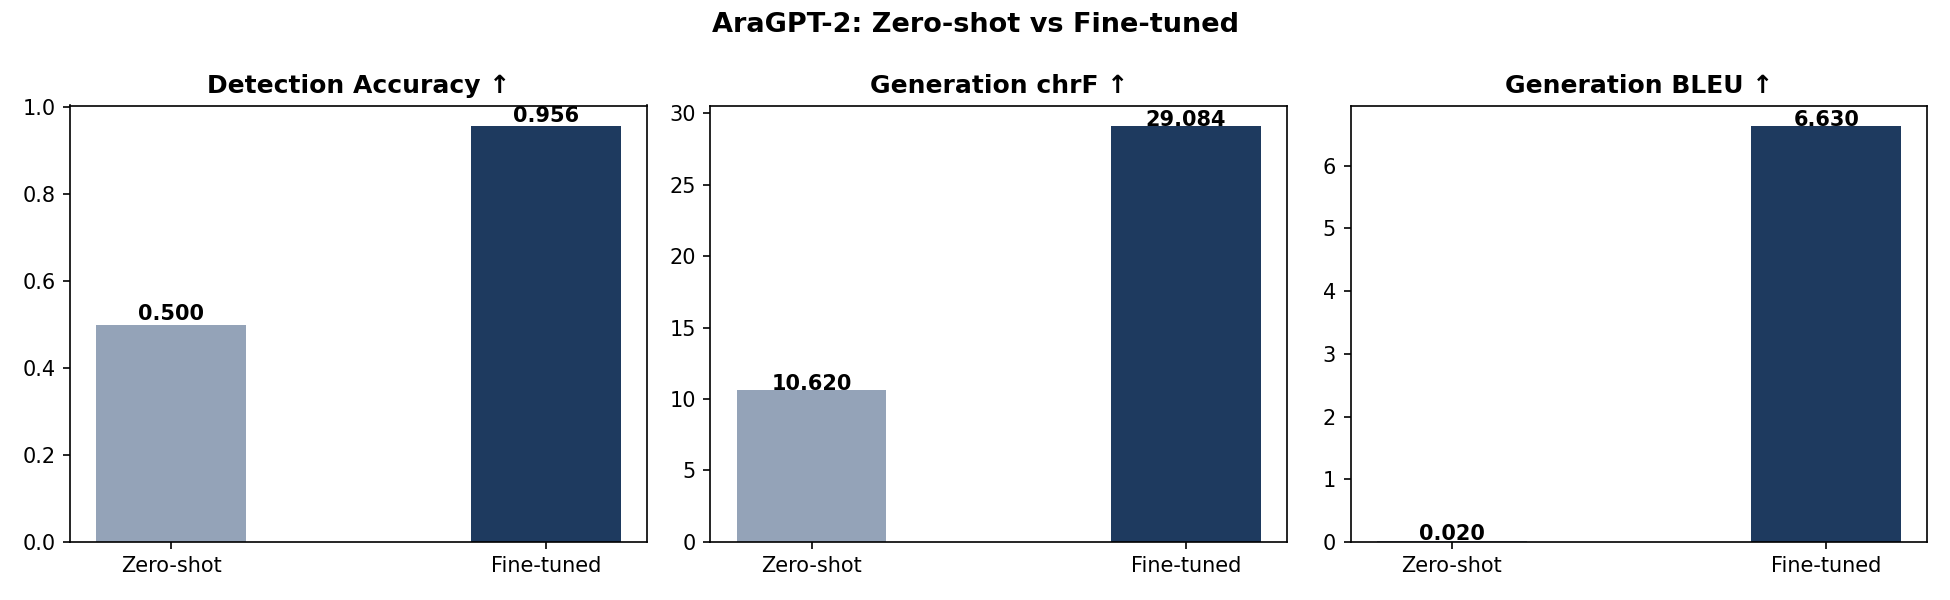
\includegraphics[width=0.65\textwidth]{full_comparison.png} \caption{Detection training curve: loss and dev accuracy over 8 epochs.} \label{fig:det_curve} \end{figure}

Fine-tuning improves detection accuracy by \textbf{+45.6 percentage points} over the zero-shot baseline and generation chrF by \textbf{+18.5 points}. The near-identical dev and test accuracy (0.956 on both) indicates that the detection model generalizes well and does not overfit to the development set.

For generation, perplexity increased from 11,851,030 (zero-shot) to 59,104,078 (fine-tuned) on the test set. We discuss this counterintuitive result in Section~\ref{sec:analysis}.

%───────────────────────────────────────────────────────────────────
\section{Analysis}
\label{sec:analysis}

\subsection{Detection Model}

\paragraph{Training dynamics.}
Training loss decreases steadily from 0.71 at epoch 1 to 0.10 at epoch 8, while development accuracy rises sharply from 0.50 at epoch 1 to approximately 0.95 by epoch 3, where it plateaus for the remainder of training. This rapid convergence suggests that the cloze-style prompt provides a strong inductive bias and that the classification signal is clearly learnable from the parallel data.
\begin{figure}[h!]
\centering
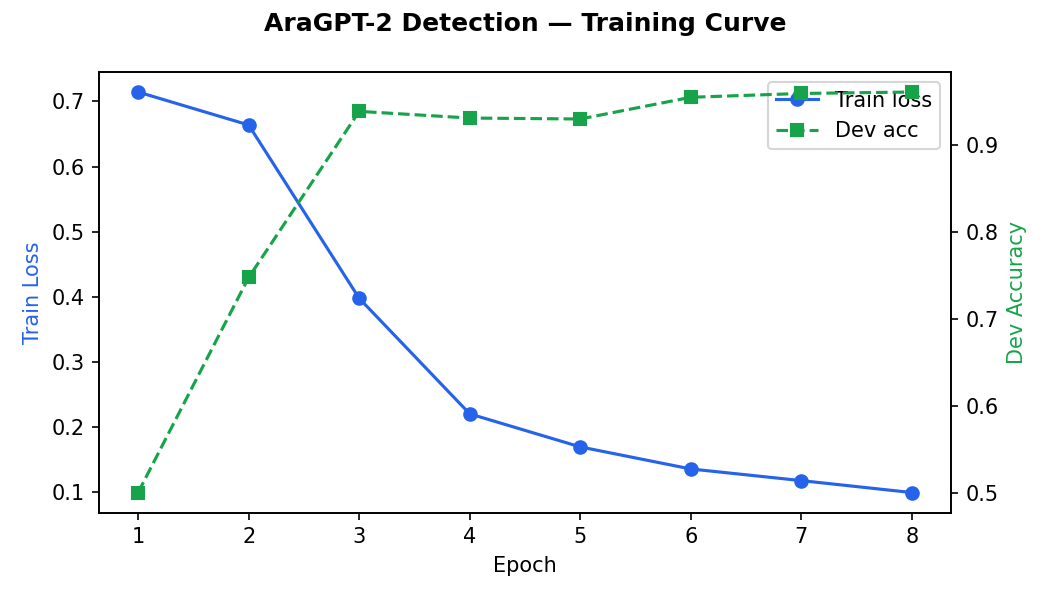
\includegraphics[width=0.55\textwidth]{training_curve.png}
\caption{Detection training curve: loss and dev accuracy over 8 epochs.}
\label{fig:det_curve}
\end{figure}
\paragraph{Error analysis.}
On the test set of 3,650 examples, the model makes 159 errors: 101 false positives (predicting \textit{correct} for an actually incorrect translation) and 58 false negatives (predicting \textit{incorrect} for a correct translation). The model is thus more prone to being over-permissive — accepting bad translations — than over-strict. This asymmetry likely reflects the hard negative sampling strategy: mismatched pairs are sometimes semantically plausible, making them genuinely hard to distinguish from correct translations.

Inspection of false positive cases reveals a consistent pattern: the model struggles when the Egyptian input is ambiguous or highly colloquial (e.g., single-word utterances like \textit{حاضر}, \textit{كويس}, \textit{أوكيه}) and the mismatched formal sentence is semantically coherent in isolation, even though it does not translate the Egyptian input. False negatives tend to occur when the correct MSA translation is unusually long or elaborate relative to the short Egyptian utterance.

\subsection{Generation Model}

\paragraph{Training dynamics.}
The generation model was trained for 5 epochs before early stopping, with training loss decreasing from approximately 2.5 at epoch 1 to 0.76 at epoch 5. Development loss reached its minimum at epoch 3 (2.39) and began increasing thereafter (2.50 at epoch 4, 2.74 at epoch 5), indicating overfitting. The best checkpoint from epoch 3 was used for all reported results.
\begin{figure}[H]
\centering
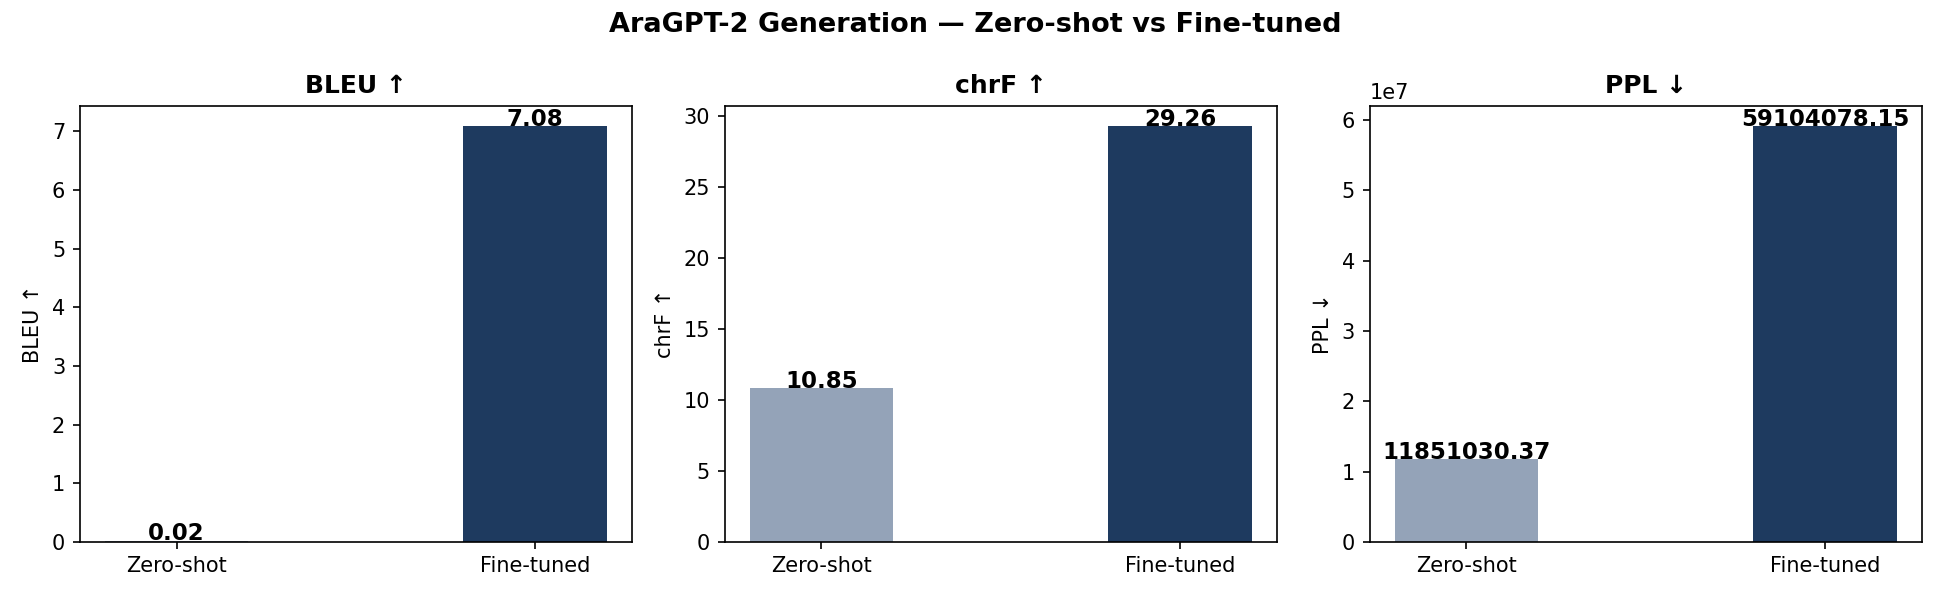
\includegraphics[width=0.65\textwidth]{generation_metrics.png}
\caption{Generation training curve: train and dev loss over 5 epochs.}
\label{fig:gen_curve}
\end{figure}
\paragraph{Qualitative comparison.}
Table~\ref{tab:gen_examples} compares zero-shot and fine-tuned generation outputs on three representative Egyptian Arabic inputs.

\begin{table}[H]
\centering
\caption{Generation examples: zero-shot vs.\ fine-tuned AraGPT-2 outputs.}
\label{tab:gen_examples}
\small
\begin{tabular}{p{3.5cm}p{5cm}p{4cm}}
\toprule
\textbf{Input (Egyptian)} & \textbf{Zero-shot output} & \textbf{Fine-tuned output} \\
\midrule
\arb{يلا فين؟}
&
\arb{مالذي جاء به من خير في هذا الشهر المبارك؟}
&
\arb{هيا، أين أنت؟}
\\
\midrule
\arb{أنا محتاج أتكلم معاكي}
&
\arb{ياام يآآإك ياروحيتي آنت لي} 
&
\arb{أحتاج أن أتحدث معك}
\\
\midrule
\arb{كنت فاكرك مش جاية}
&
\arb{يااللي ما انخطبتك} 
&
\arb{كنت أذكرك، لستِ قادمة}
\\
\bottomrule
\end{tabular}
\end{table}

The zero-shot model consistently drifts into unrelated web content — forum threads, 
religious text, social media fragments — reflecting the broad Arabic web distribution 
it was pretrained on. The fine-tuned model produces concise, on-topic MSA outputs 
that are semantically related to the Egyptian input and grammatically correct.

However, the fine-tuned model is not perfect. The third example 
(\arb{كنت فاكرك مش جاية} → \arb{كنت أذكرك، لستِ قادمة}) 
captures the sentiment but introduces a slight structural shift: the gold 
translation (\arb{ظننت أنكِ لن تأتي}) uses the verb 
\arb{ظن} (to think/assume) which better captures the nuance of 
\arb{فاكر} in context. This illustrates a broader limitation: the 
model often paraphrases correctly at the surface level but misses fine-grained 
pragmatic or aspectual nuances.

\paragraph{Perplexity anomaly.}
The increase in test perplexity from 11,851,030 (zero-shot) to 59,104,078 (fine-tuned) requires explanation. Perplexity measures how well a language model predicts the \textit{raw test token sequence} — not how well it translates. After fine-tuning, the model assigns high probability to MSA target tokens following the prompt, but the test perplexity is computed over the full sequence including the Egyptian prompt tokens, which the fine-tuned model now finds less probable under its updated distribution. This distribution shift — away from general Arabic web text toward the narrow parallel translation domain — is the root cause. The chrF and BLEU improvements confirm that translation quality improves substantially despite the perplexity increase, which is a known limitation of using perplexity as a proxy for generation quality in fine-tuned conditional models \cite{zhang2021}.

\subsection{Comparison with Hernandez and Naik}

Table~\ref{tab:comparison} places our results alongside those of the Stanford framework we extend.

\begin{table}[H]
\centering
\caption{Comparison with Hernandez and Naik \cite{hernandez2025}.}
\label{tab:comparison}
\begin{tabular}{llcc}
\toprule
\textbf{Project} & \textbf{Task} & \textbf{Zero-shot} & \textbf{Fine-tuned} \\
\midrule
Hernandez \& Naik & Slang detection (Acc) & 0.500 & 0.965 \\
\textbf{SlangGPT (ours)} & Dialect detection (Acc) & 0.500 & \textbf{0.956} \\
\midrule
Hernandez \& Naik & Slang generation (chrF) & — & 41.9 \\
\textbf{SlangGPT (ours)} & Dialect generation (chrF) & 10.62 & \textbf{29.08} \\
\bottomrule
\end{tabular}
\end{table}

Our detection result (0.956) closely matches theirs (0.965), demonstrating that the cloze-style prompting formulation transfers effectively from English slang to Arabic dialect. Our generation chrF (29.08) is lower than their sonnet generation chrF (41.9), which is expected: sonnet generation conditions on three lines of the same author and benefits from strong stylistic regularity, whereas our generation task requires cross-register translation between two structurally different language varieties with significant lexical and morphological divergence.

%───────────────────────────────────────────────────────────────────
\section{Conclusion}

In this project, we investigated how a pretrained AraGPT-2 model can be adapted to Egyptian Arabic dialect processing through fine-tuning. Extending the framework of Hernandez and Naik \cite{hernandez2025} to the Arabic setting, we fine-tuned AraGPT-2 for dialect-to-MSA generation and dialect translation detection on a parallel corpus of 18,250 Egyptian Arabic / MSA sentence pairs.

Our results show that task-specific fine-tuning substantially improves performance on both tasks. The detection model achieves 0.956 accuracy on both development and test sets, compared to a 0.500 zero-shot baseline — a +45.6 point improvement consistent with the +46.5 point improvement reported by Hernandez and Naik for English slang detection. The generation model achieves chrF of 29.08 and BLEU of 6.63, compared to zero-shot baselines of 10.62 and 0.02, demonstrating that AraGPT-2 can learn to map Egyptian dialect to formal MSA even from a moderately sized parallel corpus.

Limitations remain. The generation model begins to overfit after epoch 3, and the fine-tuned perplexity is higher than zero-shot due to distribution shift — a known artifact of conditional fine-tuning. The detection model is more prone to false positives than false negatives, particularly on ambiguous short utterances. Future work could explore larger and more diverse Egyptian Arabic corpora, encoder-decoder architectures (e.g.\ AraT5 \cite{nagoudi2022}) which are better suited to translation tasks than decoder-only models, and structural constraints such as morphological agreement checking to improve translation precision.

%───────────────────────────────────────────────────────────────────
\section*{Team Contributions}

\textbf{Abdelrahman Ahmed} — Implemented the detection model training pipeline, cloze-style prompt formulation, hard negative sampling strategy, and error analysis. Contributed to model evaluation and report writing.

\textbf{Adham Ashraf} — Built and curated the Egyptian Arabic / MSA dataset (\texttt{AdhamAshraf/egyptian-2-arabic}), implemented the data preprocessing pipeline, and led generation model training and inference. Built the Flask web application. Contributed to report writing.

\textbf{Ahmed Fekry} — Implemented evaluation scripts (chrF, BLEU, perplexity, accuracy), baseline evaluation, and visualization. Contributed to the analysis section and report writing.

%───────────────────────────────────────────────────────────────────
{\small
\bibliographystyle{unsrt}
\bibliography{references}
}
\end{document}
